% Article type supporting font formatting
\documentclass[a4paper,12pt]{extarticle}

% Define .tex file encoding
\usepackage[utf8]{inputenc}

% Norwegian language support
%\usepackage[norsk]{babel}     

% Indent first paragraph in section
\usepackage{indentfirst}

% Allows mathbb in tex file
\usepackage{amsfonts} 

\usepackage{lmodern,textcomp}

% Margin defining packagejjjj

% For quotations
\usepackage{csquotes}

% Better bibliography 
\usepackage[square,numbers]{natbib}

% For use of graphics in document
\usepackage{graphicx}         

% Allows multi-line comments in tex file
\usepackage{verbatim}         

% Allows math in tex file 
\usepackage{amsmath}          

% Allows math symbols in tex file
\usepackage{amssymb}          

% Allows use of physics shortcut functions
%\usepackage{physics}          

% Verbatim env with LaTeX commands
\usepackage{alltt}            

% Allows \begin{figure}[H]
\usepackage{float}

% Adds labeling list to the report
\usepackage{scrextend}
\addtokomafont{labelinglabel}{\ttfamily}

% Necessary for defining colours
\usepackage{xcolor}            
\definecolor{linkgreen}{rgb}{0,.5,0}
\definecolor{linkblue}{rgb}{0,0,.5}
\definecolor{linkred}{rgb}{.5,0,0}
\definecolor{blue}{rgb}{.13,.13,1}
\definecolor{green}{rgb}{0,.5,0}
\definecolor{red}{rgb}{.9,0,0}

% Hyperlinks in document
\usepackage{hyperref}  
\hypersetup{
  colorlinks=true,     % True for colored links
  linktoc=all,         % True for table of contents links
  linkcolor=linkblue,  % Colour for links
  urlcolor=linkgreen,  % Colour for URLs
  citecolor=linkred    % Colour for citations
}

% Listing package for code examples
\usepackage{listings}         
\lstset{
  language=C++,                % Set language to C++
  showspaces=false,            % Don't show space chars
  showtabs=false,              % Don't show tab chars
  breaklines=true,             % Break long lines of code
  showstringspaces=false,      % Don't show spaces in strings
  breakatwhitespace=true,      % Break at white space only
  commentstyle=\color{green},  % Set colour for comments
  keywordstyle=\color{blue},   % Set colours for keywords
  stringstyle=\color{red},     % Set colour for strings
  basicstyle=\ttfamily,        % Set basic style
  tabsize=2                    % Set tabsize
}

% Referencing, last for compatibility reasons
\usepackage[noabbrev]{cleveref}

% Command to set two lines under text
\newcommand{\uunderline}[1]{\underline{\underline{#1}}}

% Command to use integral with limits
\newcommand{\Int}{\int\limits}    

% Command to use double integral with limits
\newcommand{\IInt}{\iint\limits}  

% Command to use triple integral with limits
\newcommand{\IIInt}{\iiint\limits}

% Command removes section numbering
\newcommand{\mysection}[2]{   
  \setcounter{section}{#1}
  \section*{#2}
  \addcontentsline{toc}{section}{#2}
}

% Command removes subsection numbering
\newcommand{\mysubsection}[2]{  
  \setcounter{subsection}{#1}
  \subsection*{#2}
  \addcontentsline{toc}{subsection}{#2}
}

% Command removes subsubsection numbering
\newcommand{\mysubsubsection}[2]{ 
  \setcounter{subsubsection}{#1}
  \subsubsection*{#2}
  \addcontentsline{toc}{subsubsection}{#2}
}

% Makes matrices look square-ish
\renewcommand*{\arraystretch}{1.5}

\usepackage{tikz}

\newcommand{\shrug}[1][]{%
  \begin{tikzpicture}[baseline,x=0.8\ht\strutbox,y=0.8\ht\strutbox,line width=0.125ex,#1]
  \def\arm{(-2.5,0.95) to (-2,0.95) (-1.9,1) to (-1.5,0) (-1.35,0) to (-0.8,0)};
  \draw \arm;
  \draw[xscale=-1] \arm;
  \def\headpart{(0.6,0) arc[start angle=-40, end angle=40,x radius=0.6,y radius=0.8]};
  \draw \headpart;
  \draw[xscale=-1] \headpart;
  \def\eye{(-0.075,0.15) .. controls (0.02,0) .. (0.075,-0.15)};
  \draw[shift={(-0.3,0.8)}] \eye;
  \draw[shift={(0,0.85)}] \eye;
  % draw mouth
  \draw (-0.1,0.2) to [out=15,in=-100] (0.4,0.95); 
  \end{tikzpicture}}

%%%%%%%%%%%%%%%%%%%%%%%%%%%%%%%%%%%%%%%
%%      Title, Author, and Date      %%
%%%%%%%%%%%%%%%%%%%%%%%%%%%%%%%%%%%%%%%
\title{Visualizing Terrain Data through Ray Tracing}
\author{Daniel Aaron Salwerowicz, Christopher Kragebøl Hagerup}
\date{\today}
%%%%%%%%%%%%%%%%%%%%%%%%%%%%%%%%%%%%%%%
%%           Start document          %%
%%%%%%%%%%%%%%%%%%%%%%%%%%%%%%%%%%%%%%%
\begin{document}
  
%%%%%%%%%%%%%%%%%%%%%%%%%%%%%%%%%%%%%%%
%%   Create the main title section   %%
%%%%%%%%%%%%%%%%%%%%%%%%%%%%%%%%%%%%%%%
\maketitle

%%%%%%%%%%%%%%%%%%%%%%%%%%%%%%%%%%%%%%%
%%      Abstract for the report      %%
%%%%%%%%%%%%%%%%%%%%%%%%%%%%%%%%%%%%%%%
% \begin{abstract} 
% Say why this report exists. Motivations behind it and what not.
% \end{abstract}

%%%%%%%%%%%%%%%%%%%%%%%%%%%%%%%%%%%%%%%
%%         ToC for the report        %%
%%%%%%%%%%%%%%%%%%%%%%%%%%%%%%%%%%%%%%%
% \tableofcontents
% \pagebreak

%%%%%%%%%%%%%%%%%%%%%%%%%%%%%%%%%%%%%%
%%  The main content of the report  %%
%%%%%%%%%%%%%%%%%%%%%%%%%%%%%%%%%%%%%%

\mysection{1}{Introduction}
Our goal in this project was to use raycasting to visualize terrain data of Bjerkvik in a 3D-space. The data was provided in the form of a text file with points, and our aim was to let user change the transfer function to visualize the volume data in different ways.

\mysection{2}{Methods}
We used GMlib and some start code made by Aleksander Pedersen to represent and render the terrain in 3D-space, and used a technique called ray casting to render the terrain to the window. Ray casting uses rays sent from camera onto every pixel of image space to represent the volume data in object space. 

In our application, we read data from file. After reading all samples stored in the file, we determine the maximum and minimum values in the x-, y- and z-axis. Using these values, we normalize all of the data through feature scaling, project it into our volume, partition the volume into samples, and determine the amount of points in each sample. WE then use the number of points in each cell to determine the color and transparency values of the cell. Formula used for transforming each coordinate of point is:

$$ x_{norm} = \frac{x - x_{min}}{x_{max}-x_{min}} * \text{Cell Count}$$

Cell count refers to number of cells along each axis (100 in our case). Sans and Ramona \cite{san_2017} defines ray casting as a technique for rendering three-dimensional shapes without having to reconstruct the data. For each pixel in the image space, a ray is cast from camera into the object space. Then it records where it meets density data of the volume and using various transfer functions renders the volume to image space. Unlike the similarly named ray-tracing, ray casting does not trace rays recursively. The benefit of using ray casting is that the work is simple and can easily be parallelized, making it ideal for a Graphics-Processing Unit (GPU).

Transfer functions can be used for various purposes, in our case we used it to dynamically change colours and transparency of the volume. GUI we have set up for that lets user choose any number of points they would like on the four colour squares and see how they change the volume as well as to reset the points and volume. Code overview for our project can be found in \cref{fig:uml}.

\begin{figure}[H]
  \centering
  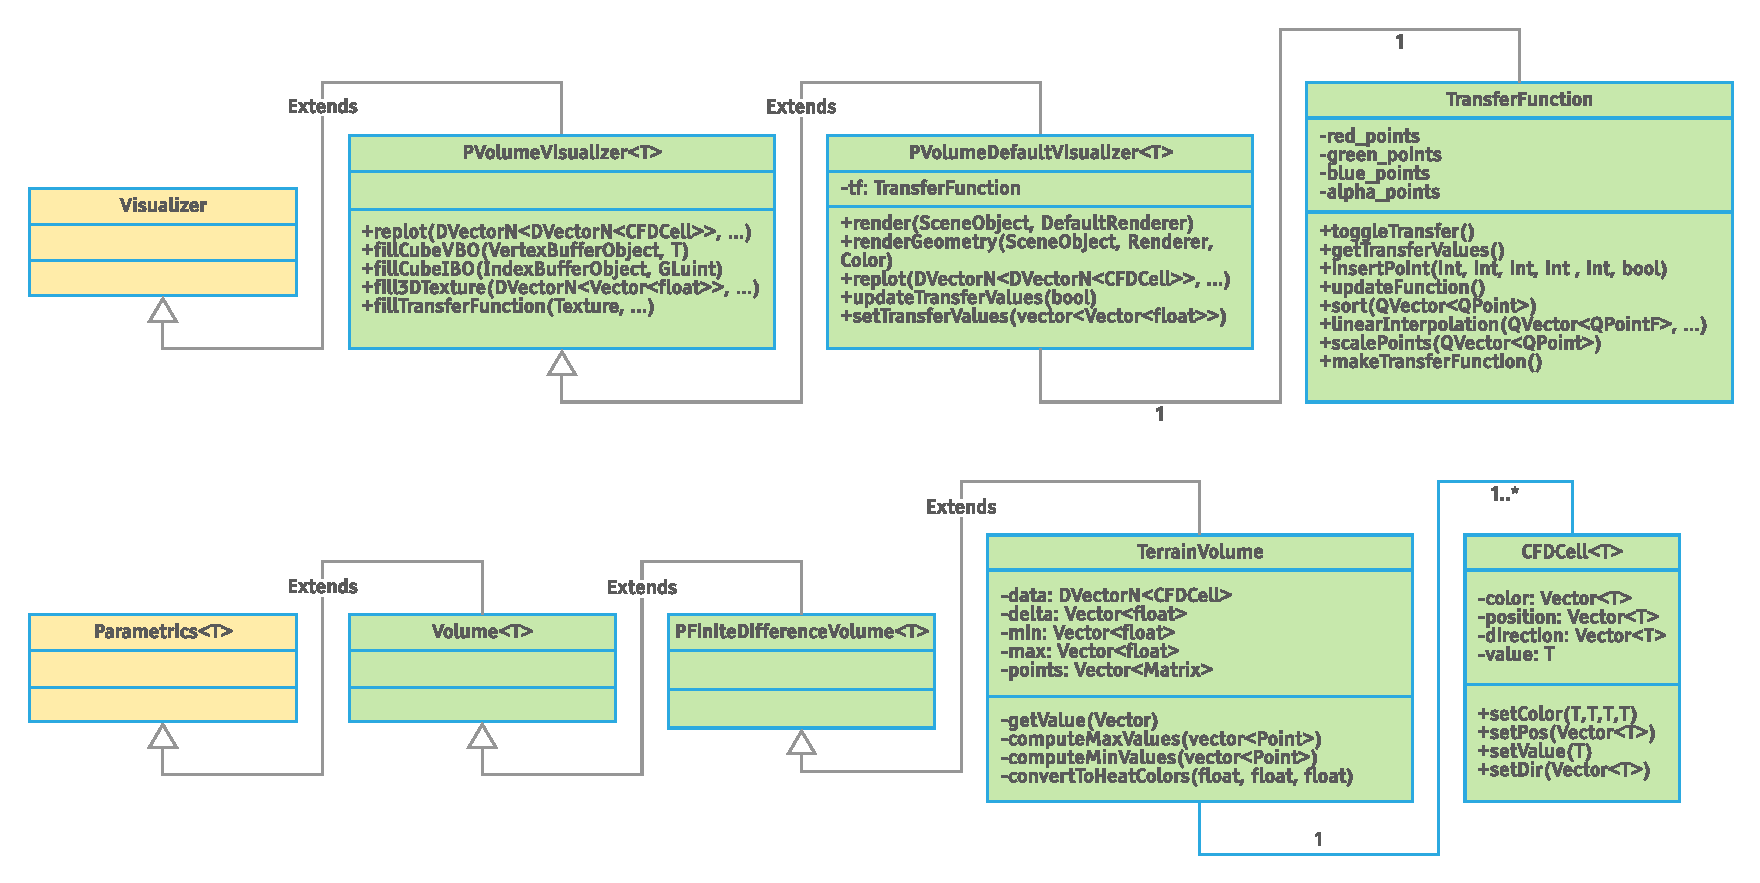
\includegraphics[width=\textwidth]{VolumeUML}
  \caption{UML class diagram our program.}
  \label{fig:uml}
\end{figure}

\mysection{3}{Results}
Our program lets users see the terrain volume and change the transfer function on the go. The visualization can be rotated and viewed from different angles to see the terrain volume better. User can also set a colour or transparency value for the volume. One can also reset the points to default value. Example of the visualized data can be seen in \cref{fig:terrainvis}.

\begin{figure}[H]
  \centering
  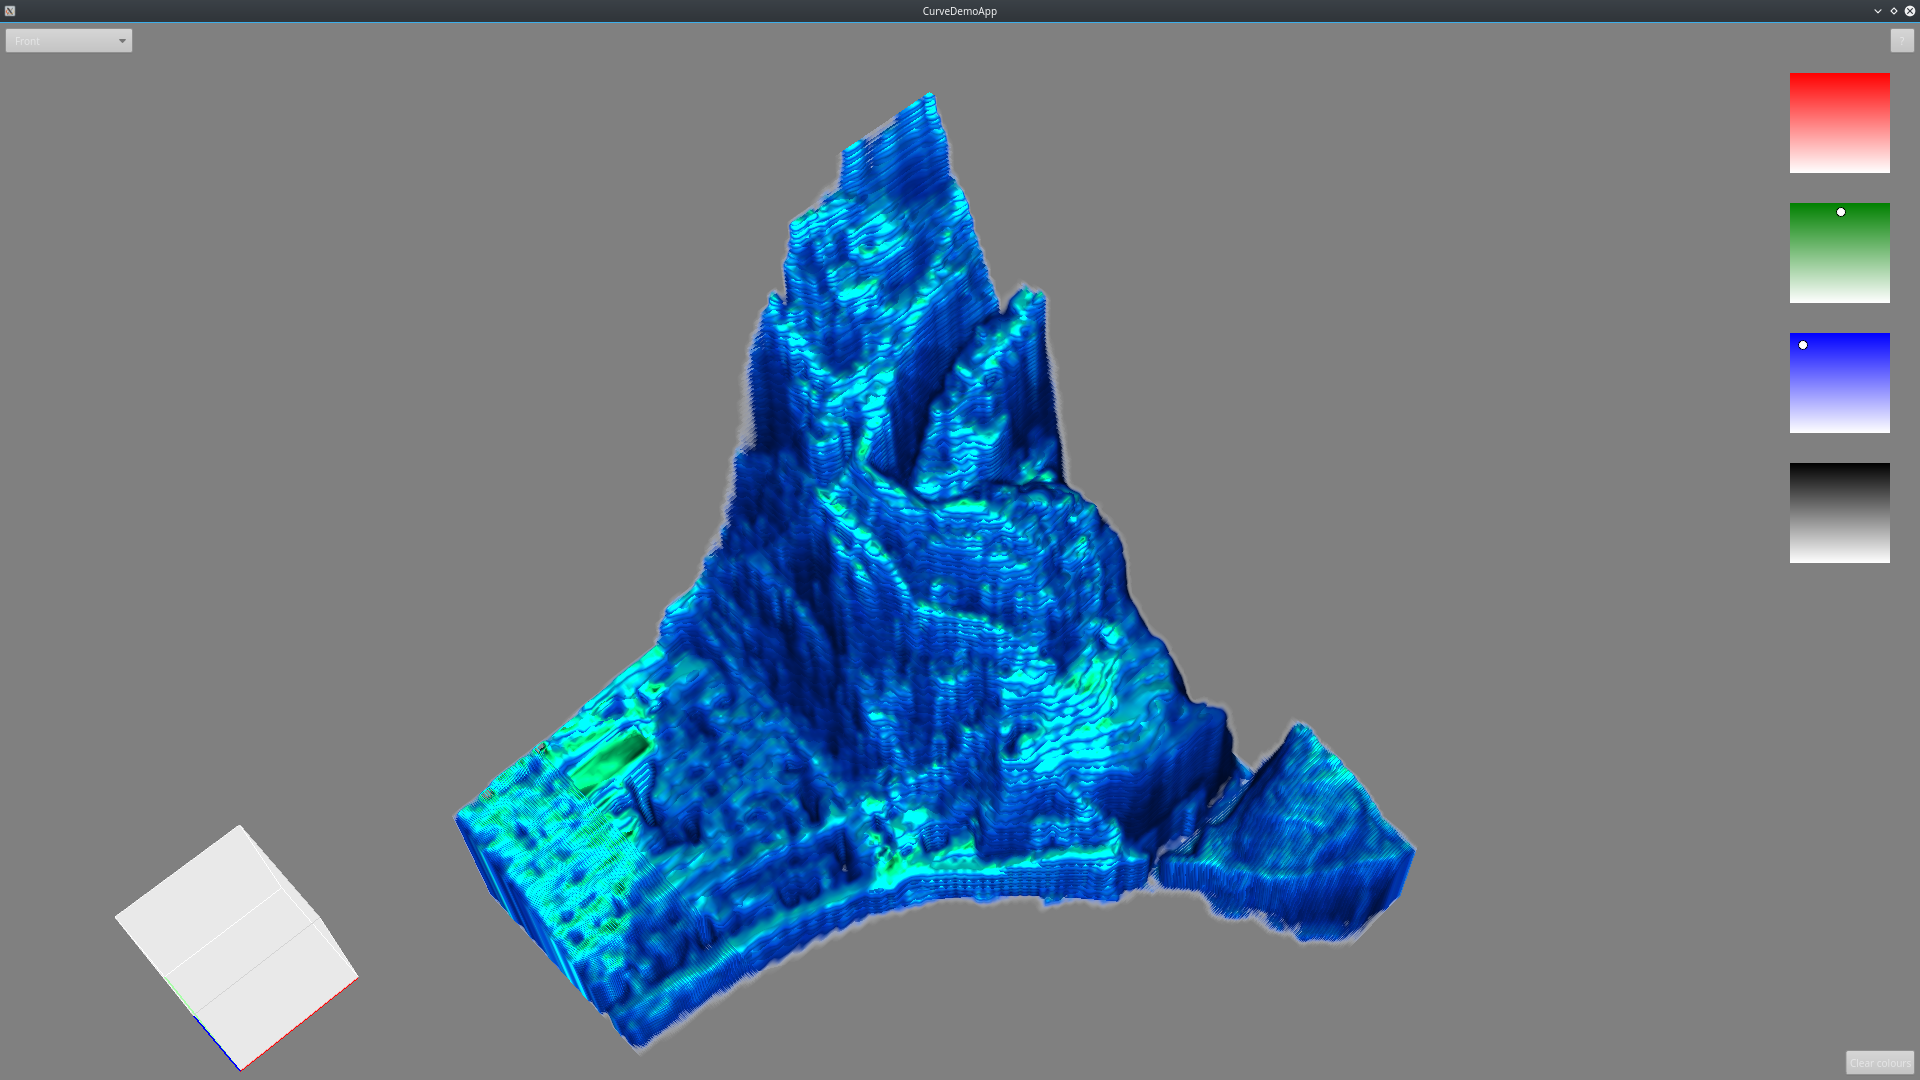
\includegraphics[width=\textwidth]{Terrainvis}
  \caption{Visualization of volume data, with brighter terrains indicating higher point density.}
  \label{fig:terrainvis}
\end{figure}

\mysection{4}{Analysis}
From our interactions with the teachers and observations, we conclude that we have managed to render the terrain properly with ray casting, although it currently is stretched quite a bit vertically. The colours are also visualized properly, according to the densities we set, but point density is the only parameter we can visualize with colours right now.

One problem we have with the data provided to us is that it's only a surface data, so we cannot properly render the volume. As we do not know the point density for cells under the surface.

\mysection{5}{Discussion}
Overall we are quite happy with the result of our work. Setting colours for the transfer function feels intuitive in our opinion (as you only need to click the colored squares to set the colors). It also runs quite fast, considering the high resolution we use. There are in total 1 million cells that our app draws and we have managed to run it with over 15 millions cells, though it takes about a minute or more to calculate and show the data. Normally reading the data, transforming it to fit our model and rendering it takes about three seconds in total, so we are quite content with the performance.

We have several opportunities for further development in our visualization. One such opportunity is to change the ray tracing and transfer function to render colours based on other things, such as the height of the map, or some other parameters. Another thing we could add if given a bit more development time is functionality for removing individual points from the transfer function (as you can only remove the points all at once right now). We originally wanted to change the colours by the use of a drop-down menu, but after discussing with Alekander, we agreed to use the coloured boxes instead, as this proved the most intuitive for the end user.

Another improvement in program is to visualize the volume realistically, so that the volume is not stretched in z-axis, as well as getting more accurate data where we know the point density under the surface, so that we can set volume transparency properly.

\mysection{6}{Acknowledgements}
We would like to thank Børre Bang and Aleksander Pedersen for giving us the initial foundations for the code of the project, and for helping us with setting up the project and volumetric visualization. As well as Jostein Bratli for helping us with GUI programming for GMlib.

We have also cooperated with our classmates Kent Arne Larsen, Olav Kjartan Larseng, and Victor Lindback and they helped us with some small problems that we had.

\mysection{7}{Bibliography}
\begingroup
\def\section*#1{}
\bibliographystyle{apa}
\bibliography{Bibliography}
\endgroup

\end{document}
